\documentclass[12pt]{thesis}

%\usepackage{amsmath}
\usepackage{tabularx}
\usepackage{ifpdf}
\usepackage{ae}

\usepackage[utf8]{inputenc}
\usepackage[english, french]{babel}
\usepackage{changepage}
%\usepackage[nottoc]{tocbibind}
\usepackage[final]{pdfpages}
\usepackage{tikz}
\usepackage{verbatim}
\usetikzlibrary{arrows,shapes}
%\usepackage{algorithm}
%\usepackage{algorithmic}
%\usepackage{vector}
\usepackage{graphicx,natbib,amssymb,lineno}
%\usepackage{latex8}
\usepackage{color}
\usepackage{subfigure}
\providecommand{\keywords}[1]{\textbf{\textit{Keywords---}} #1}
\def \cind {\,\bot\hspace{-.50em}\bot\,}
\def \un {\hbox{\rm 1\hskip -2.4pt l}}

\renewcommand{\baselinestretch}{1.5}

\captionheaderfont{\sl\bfseries}
\captionbodyfont{\sl}
\renewcommand{\tableshortname}{Table}
\renewcommand{\figureshortname}{Figure}
\chapapp{\chaptername}

\newcommand{\so}{\mbox{so}}

\newtheorem{theorem}{Th\'eor\`eme}
\newtheorem{definition}{D\'efinition}
\newtheorem{lemma}[theorem]{Lemme}
\newtheorem{examp}{Exemple}
\newtheorem{corol}[theorem]{Corollaire}

\textheight=600pt
\textwidth=450pt
\marginparwidth=1pt
\topmargin=10pt
\oddsidemargin=1pt
\marginparsep=1pt

\newcommand{\reportTitle} {%
  %\textsc{Graduation Project}
  \textsc{A Graduation Project}
}

\newcommand{\reportAuthor} {%
  First Name \textsc{Last Name}%
}

\newcommand{\reportSubject} {%
  My Title
}

\newcommand{\dateSoutenance} {%
  12/06/2024%
}

\newcommand{\studyDepartment} {%
  Host compagny
}

\newcommand{\ESAM} {
 Higher School of Agriculture of Mograne
}

%\newcommand{\codePFE} {% Reference
%  Code PFE%
%}

\newcommand{\anneeuniv}{
2023-2024}


%\frenchbsetup{StandardLists=true} 
\usepackage{titlesec}
\titleformat{\chapter}[display]
  {\centering\normalfont\huge\bfseries}{\chaptertitlename\ \thechapter}{14pt}{\Huge}

\begin{document}
% -----------------------------
% PAGE DE GARDE
% -----------------------------
\frontmatter
\title{\vspace{-5cm}

\begin{adjustwidth}{-1cm}{-1cm}
\begin{center}
    \begin{tabular}{p{4.5cm}p{7cm}p{6cm}}
    \centering
\includegraphics[width=0.8\linewidth]{universite-carthage.PNG} \\ 
    \scriptsize Carthage University& 
    \centering
\includegraphics[width=0.6\linewidth]{embleme.jpg} \\ \scriptsize\textbf{\textbf{Tunisian Republic}}\\ \scriptsize Ministry of Higher Education and Scientific Research \& Ministry of Agriculture, Water Resources and Fisheries  & 
    \centering
\includegraphics[width=0.5\linewidth]{ModelePFE_latex ESAM/IRESALOGO.png}\\ \scriptsize Institution of Agricultural Research and Higher Education \\
    \end{tabular}
\end{center}
\end{adjustwidth}


\begin{center}
    \begin{tabular}{p{7cm}}
    \centering
    
\includegraphics[width=0.4\linewidth]{ModelePFE_latex ESAM/ESAMLOGO.png}\\
    \footnotesize \textbf{Higher School of Agriculture of Mograne}\\
    \end{tabular}
\end{center} 

\begin{center}\small \textbf{\textit{Graduation Project Report submitted to obtain the degree of}} \end{center}
\begin{center} \normalsize National Diploma of Engineering in ....... 
\end{center}

\vspace{-2cm}}
\vspace{-2cm}
\author{
\large \reportAuthor
\vspace{-2cm}}
\date{\begin{center}
\rule{0.5\textwidth}{.4pt} \\
 \Large \reportSubject \\
\rule{0.5\textwidth}{.4pt}\\
\normalsize Defended on~\dateSoutenance~ in front of the committee composed of :\end{center}
\vspace{-1cm}}

\institution{\begin{center}
\begin{itemize}
  \item Last name and first name of member 1,  Grade, Affiliation (President)
  \item Last name and first name of member 2,  Grade, Affiliation (Reviewer)
  \item Last name and first name of member 3,  Grade, Affiliation (Company supervisor)
  \item Last name and first name of member 4,  Grade, Affiliation (University supervisor)
  \end{itemize}
%\textbf{\textit{End of studies internship completed at}}\\
\end{center}
%\begin{minipage}{7cm}\begin{center}\small \textbf{\studyDepartment} \end{center}\end{minipage}  \begin{minipage}{7cm}\begin{center}\includegraphics[width=0.4\linewidth]{ModelePFE_latex ESAM/logo.jpg} \end{center}\end{minipage}
%\vspace{0.1cm}
\begin{center}\small Academic year \anneeuniv \end{center}
}



%\dedication{\begin{flushright}\textit{\small{A mes parents, Sameh, Aichoucha et Yassine}}\end{flushright}}
%\uppertitleback{ENIT- Ut\'e de Tunis El Manar}
%\middletitleback{Publication Data:\\
%\tt F. Phidias Fanstord\\
%Fighting Fire with Fire\\
%Festooning French Phrases\\
%Fanstord: Fanstord University Press\\
%ISBN 0-4850}}
%\lowertitleback{Copyright $\copyright$ 1993 Phoney-Baloney}

\dedication{\begin{flushright}\textit{\small{Write your dedication...}}\end{flushright}}


\maketitle

\chapter*{\textit{Thanks}}
 \textit{
And put your thanks here. \\Lorem ipsum dolor sit amet, consectetur adipisicing elit, sed do eiusmod
tempor incididunt ut labore et dolore magna aliqua. Ut enim ad minim veniam,
quis nostrud exercitation ullamco laboris nisi ut aliquip ex ea commodo
consequat.}

\renewcommand{\abstractname}{Abstract}
\begin{abstract}

Put here an absract for the report\\
An abstract is a self-contained, short, and powerful statement that describes a larger work. An abstract of scientific work may contain the scope, purpose, results, and contents of the work. An abstract is not a review, nor does it evaluate the work being abstracted. While it contains key words found in the larger work, the abstract is an original document rather than an excerpted passage.

250 mots MAXIMUM.

\keywords{Insert some keywords}
\end{abstract}

\renewcommand{\contentsname}{Table of Contents}
\tableofcontents

\renewcommand{\listfigurename}{List of Figures}
\listoffigures

\renewcommand{\listtablename}{List of Tables}
\listoftables


%\chapter{Preface}

\mainmatter




%\tableofcontents
\chapter*{Introduction}
\addcontentsline{toc}{chapter}{Introduction} 


\renewcommand{\chaptername}{Chapter} 
\chapter{Chapter One}

And your chapter one goes here and you must cite your bibliography like this \cite{schaeffer99}, \cite{jenkins2004}, \cite{caillois1}.

Here is a math formula in the line $x^2=\log(x)$ and another in the middle
$$x^2=\displaystyle\frac{2}{3}$$
also we can cite the equation (\ref{eq1})
\begin{equation}
x^2=\displaystyle\frac{2}{3} \label{eq1}
\end{equation}
\section{Paragraph 1}

The graphic of the figure \ref{fig1}

\begin{figure}[h]
\centering
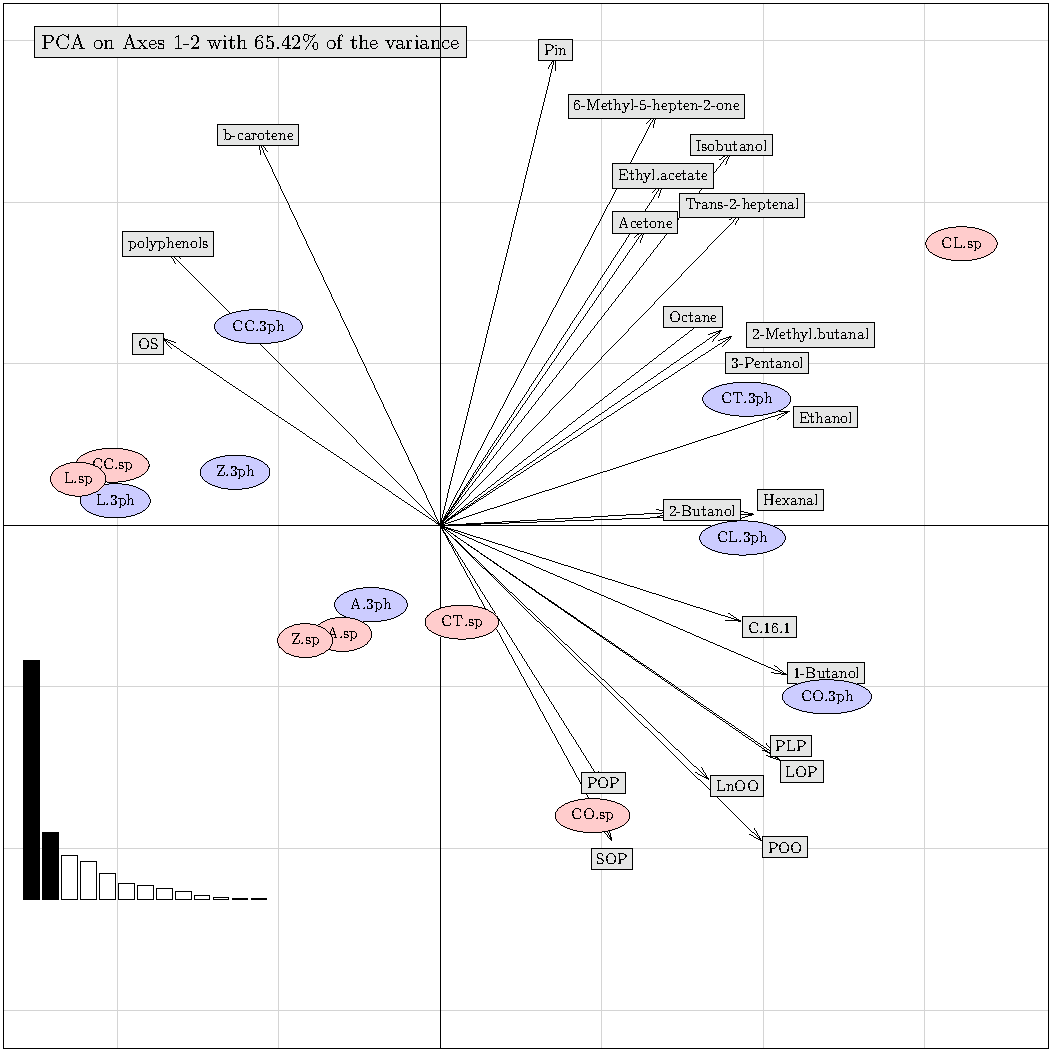
\includegraphics[scale=.5]{acp1}
\caption{Mon graphe \label{fig1}}
\end{figure}

\begin{table}[]
    \centering
    \begin{tabular}{|c||c|c|c|c|}
    \hline
        Variétés & Ph & Poids& Taille& X \\ \hline
        Chemlali & 1.4 & ... & ... &... \\ \hline
        ... & ... & ... &...  &... \\ \hline
    \end{tabular}
    \caption{Descriptive Statistics}
    \label{tab:my_label}
\end{table}



\bibliographystyle{abbrvnat}
%\bibliographystyle{apalike}
 \bibliography{Biblio}


\end{document}
